%!TEX root = ../rapport.tex
\chapter{Analyse, conception, réalisation et tests de la partie cliente}
\label{cha:analyse_client}

Ce chapitre regroupe les différentes parties qui ont été effectuées pour la partie cliente du système. Il s'agit donc de l'application \emph{\gls{ipad}} qui sera analysée. Ensuite une conception plus détaillée sera faite d'une part pour mieux se faire comprendre par le client et d'une autre part pour faciliter la partie suivante qui est la réalisation. Pour terminer ce chapitre, les résultats des tests effectués sur le client seront reportés.

\section{Analyse} % (fold)
\label{sec:analyse_client}
Vous trouverez ci-dessous l'analyse qui a été faite sur le développement \emph{\gls{ios}} ou sur le principe du format \emph{\gls{json}}. D'autres points ont été analysés afin de se faire une première idée sur les possibilités qui s'offriront pour le développement.
\subsection{Concepts de développement sur iOS} % (fold)
\label{sub:concepts_de_d_veloppement_sur_ios}

\subsubsection{Protocoles \& Delegates}
Les \emph{protocoles} et les \emph{delegates} sont intimement liés lorsqu'on développe en \emph{\gls{obj-c}}.

\medskip 

Un protocole permet de déclarer des méthodes qui peuvent être implémentées par une classe. Cela ressemble fortement aux interfaces dans le monde \emph{\gls{java}}. Le code \ref{lst:protocol} montre comment déclarer un protocole alors que le code \ref{lst:protocol2} comment suivre ce protocole. On dit que la classe qui suit un protocole est son délégué.

\begin{lstlisting}[language={C}, caption={Déclarer un protocole Printing}, label={lst:protocol}]
@protocol Printing
	-(void) print;
@end
\end{lstlisting}

\begin{lstlisting}[language={C}, caption={Suivre le protocole Printing}, label={lst:protocol2}]
#import <Foundation/NSObject.h>
#import "Printing.h"

@interface Fraction: NSObject <Printing> {
    int numerator;
    int denominator;
}
\end{lstlisting}
\subsubsection{Storyboard}
\emph{Storyboard} est une nouvelle manière de dessiner ou designer les interfaces que l'on crée dans \emph{\gls{xcode}}. 

\medskip

Cela permet également, et c'est là un point très fort, de définir les différentes interactions qui existent entre les interfaces de notre application. La figure \ref{gra:storyboard} montre un exemple de storyboard tiré du site internet \cite{online:RayWenderlich}.

\begin{figure}[H]
    	\centering
    	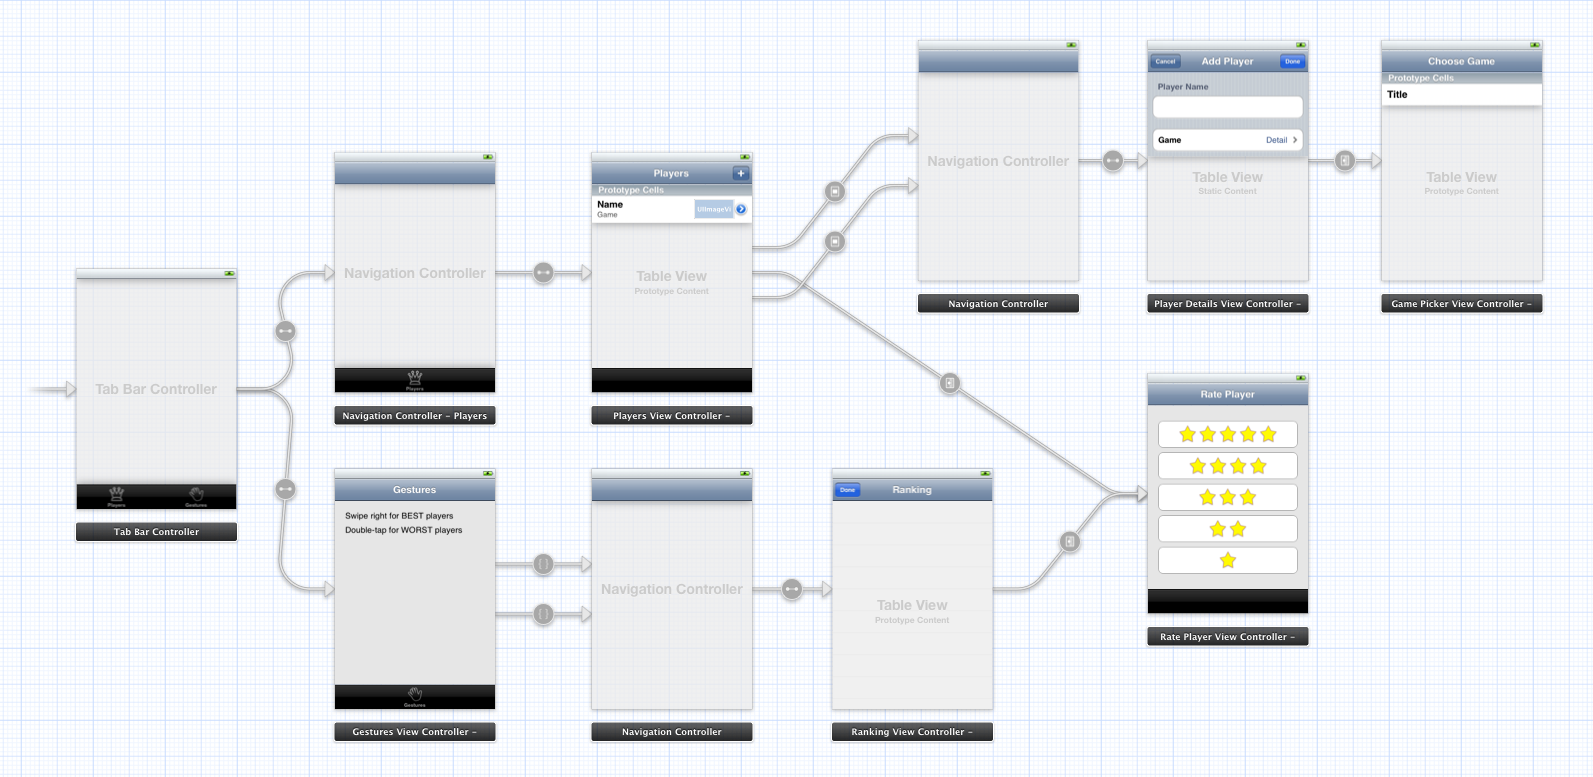
\includegraphics[width=\textwidth]{00_media/storyboard.png}
    	\caption{Exemple de Storyboard tiré du site \cite{online:RayWenderlich}}
    	\label{gra:storyboard}
\end{figure}
% subsection concepts_de_d_veloppement_sur_ios (end)

\subsubsection{ARC}
Depuis \emph{\gls{ios}} 5, \emph{\gls{arc}} permet de ne plus nous soucier des références en effectuant des \emph{retain} ou des \emph{release}.

\medskip

Ce n'est pas exactement un \emph{Garbage collector} \emph{(Ramasseur de miettes)} qui est par exemple effectué pour du \emph{\gls{java}}. En effet, les \emph{retain} ou les \emph{release} que l'on insérait avant sont simplement ajoutés automatiquement. 

\medskip

C'est pour cette raison qu'il est d'ailleurs toujours obligatoire, comme le montre le code \ref{lst:arc} tiré d'un exemple sur le site \cite{online:LongWeekendLLC}, de créer un \emph{Pool Auto Release} dans le \emph{Main} d'un programme lorsqu'on crée une application.
\begin{lstlisting}[language={C}, caption={Autorelease Pool tiré d'un exemple du site \cite{online:LongWeekendLLC}}, label={lst:arc}]
int main(int argc, char *argv[])
{
  @autoreleasepool {
    return UIApplicationMain(argc, argv, nil, NSStringFromClass([ExampleAppDelegate class]));
  }
}
\end{lstlisting}

\subsubsection{Gestures recognizers}

Les reconnaissances de gestes sur une \texttt{UIView} ou une de ses sous-classes sont disponibles depuis la version 3.2 \emph{\gls{ios}}. La liste ci-dessous décrit chaque \emph{Gesture Recognizer}.

\bigskip

\begin{itemize}
  \item \texttt{UITapGestureRecognizer} permet de détecter 1 ou plusieurs tapes sur l'écran. On peut définir le nombre de tapes requises.
  \item \texttt{UIPinchGestureRecognizer} permet de détecter lorsque 2 doigts vont dans le sens contraire comme par exemple pour agrandir un objet.
  \item \texttt{UIRotationGestureRecognizer} permet de détecter lorsque 2 doigts sont opposés et font un mouvement circulaire comme par exemple changer la rotation d'une forme.
  \item \texttt{UISwipeGestureRecognizer} permet de détecter une glissement avec un ou plusieurs doigts sur un objet dans une direction qui est définit par nos propres soins.
  \item \texttt{UIPanGestureRecognizer} permet de détecter lorsqu'un utilisateur a cliqué sur un objet et désire le déplacer. On peut également définir le nombre de doigts.
  \item \texttt{UILongPressGestureRecognizer} permet de détecter lorsqu'un utilisateur clique une certaine durée sur un objet. Cette durée peut être définie.
\end{itemize}

\bigskip

Il est possible d'ajouter une reconnaissance de geste sur une \texttt{UIView} grâce à la méthode \texttt{addGestureRecognizer:}. 

\medskip

Le code \ref{lst:grexemple} en donne un exemple. En effet, on ajoute un \texttt{UITapGestureRecognizer} sur la vue principale ce qui aura comme conséquence d'appeler la méthode \texttt{tapOnScreen:} lorsque l'utilisateur aura tapé 2 fois sur l'écran.

\begin{lstlisting}[language={JAVA}, caption={Exemple d'ajout gesture recognizer}, label={lst:grexemple}]
UITapGestureRecognizer *tapView = [[UITapGestureRecognizer alloc] initWithTarget:self action:@selector(tapOnScreen:)];
tapView.numberOfTapsRequired = 2;
[self.view addGestureRecognizer:tapView];
\end{lstlisting}

Le code \ref{lst:tapOnScreen} montre comment déclarer les méthodes qui traîte les reconnaissances de gestes.

\begin{lstlisting}[language={JAVA}, caption={Exemple de traitement d'un geste}, label={lst:tapOnScreen}]
- (void)tapOnScreen:(UITapGestureRecognizer*)gesture {
    NSLog(@"Tap on the screen");
}
\end{lstlisting}

Il est également possible de spécifier si la reconnaissance doit être détectée ou non grâce à la méthode du \emph{delegate} de \emph{UIGestureRecognizerDelegate} reportée au code \ref{lst:shouldReceiveTouch}. Cette méthode retourne alors un \emph{BOOL}.
\begin{lstlisting}[language={JAVA}, caption={Gesture shouldReceiveTouch}, label={lst:shouldReceiveTouch}]
- (BOOL)gestureRecognizer:(UIGestureRecognizer *)gestureRecognizer shouldReceiveTouch:(UITouch *)touch;
\end{lstlisting}

\subsection{Utilisation des ressources sur l'iPad} % (fold)
\label{sub:utiliser_des_ressources_de_l_ipad}
Lorsque l'utilisateur veut importer une photo d'un plan dans l'application, il faut que cela se fasse facilement. Il y a plusieurs moyens de le faire. Voici une liste qui regroupe des idées pour cette partie : 

\medskip

\begin{itemize}
	\item Sélectionner une photo dans la librairie de photos sur l'\emph{\gls{ipad}}
	\item Sélectionner une photo sur un disque qui permet de partager (DropBox, Wuala, ...)
	\item Prendre directement une photo depuis l'application
\end{itemize}

\medskip

Une analyse des différentes possibilités a été faite, ci-dessous, afin d'avoir déjà une idée sur la complexité de mise en place et le niveau de difficulté de son intégration dans une application \emph{\gls{ipad}}.

\subsubsection{Photos Library}
\emph{\gls{ios}} propose dans sa couche \emph{UIKit} une classe \emph{UIImagePickerController} afin de permettre à l'utilisateur de choisir une photo ou une vidéo sauvée sur des appareils tels que l'iPhone, l'iPod ou l'\emph{\gls{ipad}} par exemple. Grâce à cette classe, on peut faire en sorte de proposer directement de prendre une photo ou une vidéo. Une documentation est disponible sur le site \cite{online:iosimagepickercontroller}.

\medskip

Pour utiliser cela, il faut suivre le protocole \emph{UIImagePickerControllerDelegate} qui propose deux méthodes : 

\begin{description}
  \item [imagePickerController:didFinishPickingMediaWithInfo:] est appelée lorsque l'utilisateur a choisi une image ou une vidéo.
  \item [imagePickerControllerDidCancel:] est appelée lorsque l'utilisateur décide de ne pas choisir d'image en quittant l'interface.
\end{description}

\medskip

Une documentation est disponible sur le site \cite{online:iosimagepickerdelegate}.


\subsubsection{Dropbox}

\emph{Dropbox} est un service qui permet de stocker des dossiers et des fichiers en ligne afin de les partager avec d'autres utilisateurs par exemple ou également pour avoir une sauvegarde en ligne.

\medskip

Il existe une \emph{API} permettant d'apporter les fonctionnalités de \emph{Dropbox} dans une application \emph{\gls{ios}}, à savoir :

\medskip

\begin{itemize}
  \item Lire et écrire de façon sécurisée
  \item Rechercher
  \item Partager
  \item Restaurer des fichiers dans des versions précédentes
\end{itemize}

\medskip

Sur le site \cite{online:dropapi}, il y a des informations concernant les concepts de l'\emph{API}, la configuration de l'application, l'authentification à un compte \emph{Dropbox} ainsi que la gestion des fichiers et des dossiers. 


\subsubsection{Appareil photo}
Il est possible d'utiliser la caméra de l'\emph{\gls{ipad}} pour prendre des photos depuis notre programme. \emph{\gls{ios}} propose cela dans sa couche \emph{AV Foundation} qui fournit une interface pour gérer et utiliser des médias audios ou visuels dans notre application. Pour cela, il faut au minimum : 

\medskip

\begin{itemize}
	\item Utiliser une instance de la classe \texttt{AVCaptureDevice} qui représente un appareil prenant une information en entrée comme la caméra ou le microphone.
	\item Utiliser une instance d'une sous-classe de classe \texttt{AVCaptureInput} pour configurer l'entrée d'une vidéo ou d'une image comme par exemple les ports.
	\item Utiliser une instance d'une sous-classe de classe \texttt{AVCaptureOutput} pour gérer le traîtement d'une vidéo ou d'une image.
	\item Utiliser une instance de la classe \texttt{AVCaptureSession} pour par exemple, présenter ce que l'utilisateur est en train de filmer.
\end{itemize}

\medskip

Apple propose sur le site \cite{online:avfoundation} un guide \emph{AV Foundation} et plus précisément pour capturer et gérer des médias.

\medskip

{\bf Note:} Il vaudrait peut être mieux utiliser simplement l'appareil photo de manière standard et ensuite parcourir la librairie sur l'\emph{\gls{ipad}} afin de choisir l'image. Cela serait beaucoup plus rapide à implémenter.
  
% subsection utiliser_des_ressources_de_l_ipad (end)

\subsection{Dessiner des formes} % (fold)
\label{sub:dessiner_des_formes}

Lorsqu'on développe en \emph{\gls{obj-c}}, il me parait important de savoir quels sont les moyens à disposition permettant de dessiner ou d'insérer des formes telles des rectangles ou des ronds.

\medskip

C'est d'après moi ainsi qu'on insérera des zones sur notre plan lors de la partie d'implémentation du client.

\medskip

Il existe plus d'une façon de dessiner des objets. Ci-dessous une liste qui me semble être intéressante.

\medskip

\begin{itemize}
  \item Utiliser des CALayer du framework QuartzCore
  \item Utiliser des UIView ou des sous-classes de UIView
  \item Utiliser des images prédéfinies
\end{itemize}

\subsection{Sauvegarde des préférences utilisateurs} % (fold)
\label{sub:sauvegarde_des_pr_f_rences_utilisateurs}
Généralement, les applications \emph{\gls{ios}} proposent de sauvegarder des préférences utilisateurs pour une application comme par exemple le nom d'utilisateur ou le mot de passe.

\medskip

Pour cela, \emph{\gls{ios}} propose deux solutions : 

\medskip

\begin{itemize}
  \item Gérer cela depuis l'application
  \item Utiliser des \emph{Bundle} pour gérer les préférences depuis les paramètres de l'appareil 
\end{itemize}

\medskip

Pour utiliser la deuxième solution, (stocker les informations dans les paramètres de l'appareil), une documentation est disponible sur le site \cite{online:iosbundle}.

\medskip

Pour utiliser les ressources depuis l'application, il existe une classe \emph{NSUserDefaults} qui est une interface permettant d'interagir avec le système.
Une documentation est disponible sur le site \cite{online:nsuserdefaults}.
% subsection sauvegarde_des_pr_f_rences_utilisateurs (end)

\subsection{RestKit Framework}
Il existe un framework permettant de faciliter le travail avec un \emph{\gls{webservice}} de type \emph{\gls{rest}}. Ce dernier s'appelle \emph{RestKit} qui est un framework pour le langage \emph{\gls{obj-c}} permettant de se concentrer davantage sur nos données que sur les détails d'envois de requête, de la gestion du parsing, etc... 

\medskip

Pour tester cet outil, j'ai reproduit la gestion du login avec le \emph{\gls{webservice}} qui a été fait avant le projet. Ceci a été fait en \emph{\gls{obj-c}}. Une documentation d'installation est disponible sur le site \cite{online:restkit}. Il est nécessaire et important de suivre correctement ce guide afin de pouvoir utiliser le framework par la suite.


% subsection  (end)


\subsection{JSON} % (fold)
\label{sub:}
Le \emph{\gls{webservice}} retourne les informations demandées au format \gls{json} \emph{(JavaScript Object Notation)}. \gls{json}  est un format de données, textuel, issu du langage \emph{\gls{javascript}}. souvent utilisé lorsqu'on travaille avec des données récupérées sur un serveur ou du moins, à distance. Ce format est facile à lire ou à écrire pour des humains.

\subsubsection{Objet JSON}
En \gls{json}, un objet est un ensemble de nom - valeur. Il commence par une accolade ouvrante (\texttt{\{}) et se termine par une accolade fermante (\texttt{\}}). La figure \ref{gra:jsonsyntax} illustre un diagramme syntaxique rendant valide un objet \gls{json}.

\begin{figure}[H]
      \centering
      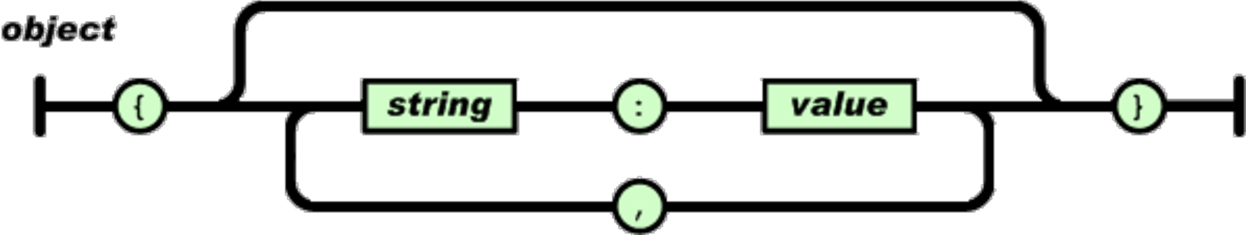
\includegraphics[width=400px]{00_media/03_objetJson.pdf}
      \caption{Diagramme syntaxique pour objet JSON tiré du site \cite{online:jsonorg}}
      \label{gra:jsonsyntax}
\end{figure}

\subsubsection{Tableau JSON}
Un tableau est une collection de valeurs. Il commence par une accolade ouvrante (\texttt{\{}) et se termine par une accolade fermante (\texttt{\}}). La figure \ref{gra:jsonsyntaxarray} illustre un diagramme syntaxique rendant valide un tableau \gls{json}.

\begin{figure}[H]
      \centering
      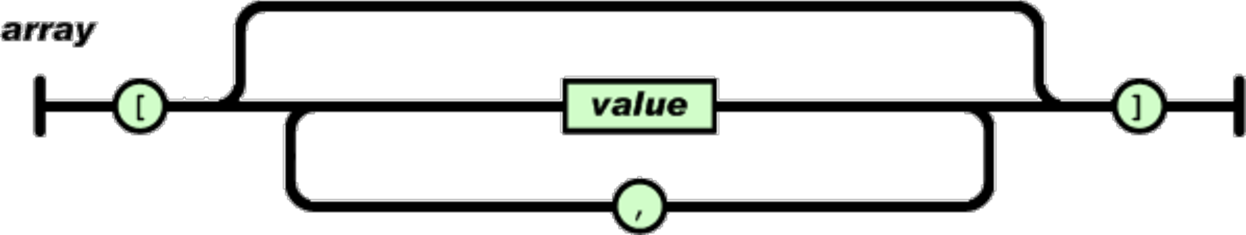
\includegraphics[width=400px]{00_media/03_arrayJson.pdf}
      \caption{Diagramme syntaxique pour array JSON tiré du site \cite{online:jsonorg}}
      \label{gra:jsonsyntaxarray}
\end{figure}
\subsubsection{Valeurs possibles}
Les valeurs peuvent être : 

\medskip

\begin{itemize}
  \item une chaîne de caractères délimité par des guillemets
  \item un nombre
  \item true
  \item false
  \item null
  \item un autre objet \gls{json}
  \item un tableau \gls{json}
\end{itemize}

\subsubsection{Exemple}
Le code \ref{lst:codeJsonExample} montre un exemple de structure \gls{json} et le code \ref{lst:codeXMLExample} son équivalent au format \emph{\gls{xml}}.
\begin{lstlisting}[language={XML}, caption={Exemple code JSON}, label={lst:codeJsonExample}]
{   "personne" :
          {     
                "prenom": "John",
                "nom" : "Doe",
                "age" : "42"
          }
}
\end{lstlisting}

\begin{lstlisting}[language={XML}, caption={Comparaison XML-JSON}, label={lst:codeXMLExample}]
<personne>
  <prenom>John</prenom>
  <nom>Doe</nom>
  <age>42</age>
</personne>
\end{lstlisting}

\subsubsection{Objectify}
Il existe un utilitaire intéressant qui permet de convertir du code \gls{json} en classe codé en \emph{\gls{obj-c}}. Cette utilitaire se nomme \emph{Objectify} et est disponible sur le site \cite{online:objectify}.

\medskip

Pour montrer de quoi est capable ce programme, j'ai repris le code \ref{lst:codeJsonExample} et le résultat de l'opération peut être visible sur le code \ref{lst:objectifya} pour le fichier \emph{header} et \ref{lst:objectifyb} pour le fichier d'implémentation.

\medskip

Comme le montre les résultats, ce programme peut nous faire gagner du temps pour concevoir les entités de notre application. Si cela est utilisé, il y aura cependant des modifications à faire au code car on peut voir que l'\emph{\gls{arc}} n'est pas utilisé puisqu'il y a des mots clefs comme \texttt{retain, release, autorelease} qui prouvent que la mémoire est gérée manuellement et non en profitant de \emph{\gls{arc}}.

\begin{lstlisting}[language={JAVA}, caption={Objectify - Resultat du fichier.h}, label={lst:objectifya}]
#import <Foundation/Foundation.h>
@interface MyClass : NSObject {
    NSString *age;
    NSString *nom;
    NSString *prenom;
}
@property (nonatomic, copy) NSString *age;
@property (nonatomic, copy) NSString *nom;
@property (nonatomic, copy) NSString *prenom;
+ (MyClass *)instanceFromDictionary:(NSDictionary *)aDictionary;
- (void)setAttributesFromDictionary:(NSDictionary *)aDictionary;
@end
\end{lstlisting}

\begin{lstlisting}[language={JAVA}, caption={Objectify - Resultat du fichier.m}, label={lst:objectifyb}]
#import "MyClass.h"
@implementation MyClass
@synthesize age = age;
@synthesize nom = nom;
@synthesize prenom = prenom;
- (void)dealloc {
    [age release], age = nil;
    [nom release], nom = nil;
    [prenom release], prenom = nil;
    [super dealloc];
}
+ (MyClass *)instanceFromDictionary:(NSDictionary *)aDictionary {
    MyClass *instance = [[[MyClass alloc] init] autorelease];
    [instance setAttributesFromDictionary:aDictionary];
    return instance;
}
- (void)setAttributesFromDictionary:(NSDictionary *)aDictionary {
    if (![aDictionary isKindOfClass:[NSDictionary class]]) {
        return;
    }
    self.age = [aDictionary objectForKey:@"age"];
    self.nom = [aDictionary objectForKey:@"nom"];
    self.prenom = [aDictionary objectForKey:@"prenom"];
}
@end
\end{lstlisting}
\subsubsection{SBJson}
\emph{SBJson}, appelé avant \emph{json-framework}, est un parser \emph{\gls{json}} pour le langage \emph{\gls{obj-c}}. Une documentation est disponible sur le site \cite{online:sbjson}.

\medskip

Un test technologique a été fait afin de voir comment fonctionnait ce framework. Pour commencer, il faut télécharger le projet disponible sur le site \cite{online:sbjson} et suivre le tutorial disponible sur le site \cite{online:sbjsonproject}. On peut ainsi insérer dans la classe avec laquelle on travaille l'import du fichier nécessaire pour employer le framework comme le montre le code \ref{lst:sbjsonimport}.

\begin{lstlisting}[language={JAVA}, caption={Import de l'interface SBJson}, label={lst:sbjsonimport}]
#import "SBJson/SBJsonParser.h"
\end{lstlisting}

Afin de tester, le code \ref{lst:codeJsonExample} a été repris dans le but d'afficher les valeurs pour chaque clef. Le code \ref{lst:testtechnosbjson} montre l'implémentation qui a été faite et le résultat peut être visible en \ref{lst:testtechnosbjsonb}.

\begin{lstlisting}[language={JAVA}, caption={Test technologique pour SBJson}, label={lst:testtechnosbjson}]
// On initialise le parser
SBJsonParser * myParser = [[SBJsonParser alloc]init];
NSString * myJSonString = @"{\"personne\" : {\"prenom\": \"John\",\"nom\": \"Doe\",\"age\": \"42\"}}";
// On utilise le parser pour creer un objet avec le string ci-dessus
NSDictionary *jsonObject = [myParser objectWithString:myJSonString error:NULL];
// On construit un dictionnaire pour la clef personne
NSDictionary* person = [jsonObject objectForKey:@"personne"];
// On affiche les elements en les appelant avec leur clef
NSLog(@"prenom:%@", [person objectForKey:@"prenom"]);
NSLog(@"nom:%@", [person objectForKey:@"nom"]);
NSLog(@"age:%@", [person objectForKey:@"age"]);
\end{lstlisting}

\begin{lstlisting}[language={JAVA}, caption={Test technologique pour SBJson - Résultat}, label={lst:testtechnosbjsonb}]
prenom:john
nom:doe
age:42
\end{lstlisting}

% section analyse (end)

